
\section{Summary and Outlook}

This chapter  is meant to be a short overview of the facts concerning
the Grid computing for HEP experiments, in particular for the
experiments at the CERN LHC. The experience gained during the LHC
operations in 2009-2011 has proven that for this community, the
existence of a well performing distributed computing is necessary
for the achievement and fast delivery of scientific results. The
existing WLCG infrastructure turned up to be able to support the
data production and processing thus fulfilling its first-plan
mission. It has been and will be continuously developing into the
future absorbing and giving rise to new technologies, like the
advances in networking, storage systems and inter-operability
between Grids and Clouds \cite{Cloud}\cite{Cloud2}.

\subsection{Data management}

Managing the real data taking and processing in
2009-2011 provided basic experience and a starting point for new
developments. The excellent performance of the network which was by
far not anticipated in the time of writing the WLCG (C)TDR shifted
the original concept of computing models based on hierarchical
architecture to a more symmetrical mesh-like scenario. In the original
design, the jobs are sent to sites holding the required data sets
and there are multiple copies of data spread over the system due to
anticipation that network will be unreliable or insufficient. It
turned out that some data sets were placed on sites and never
touched.

Based on the existing excellent network reliability and growing
throughput, the data models start to change along a dynamical
scenario. This includes sending data to a site just before a job
requires it, or reading files remotely over the network, use remote
(WAN) I/O to the running processes. Certainly, fetching over the
network one needed data file from a given data set which can contain
hundreds of files is more effective than a massive data sets
deployment and will spare storage resources and bring less network
load.

The evolution of the data management strategies is ongoing. It goes
towards caching of data rather than strict planned placement. As
mentioned, the preferences go to fetching a file over the network
when a job needs it and to a kind of intelligent data pre-placement.
The remote access to data (either by caching on demand and/or by
remote file access) should be implemented.


\subsection{Network}
%
To improve the performance of the WLCG-operated network
infrastructure, the topology of LHC Open Network Environment (LHCONE
\cite{LHCONE}) is being developed and built. This should be complementary to
the existing OPN infrastructure providing the inter-connectivity
between Tier-2s and Tier-1s and between Tier-2s themselves without
putting an additional load on the existing NREN infrastructures. As
we learned during the last years, the network is extremely important
and better connected countries do better.


\subsection{Resources}

During the 2010 data taking the available resources
were sufficient to cover the needs of experiments, but during 2011
the computing slots as well as the storage capacities at sites
started to be full. Since the experience clearly shows that delivery
of the Physics results is limited by resources, the experiments are
facing a necessity of more efficient usage of existing resources.
There are task forces studying the possibility of using the next
generations computing and storage technologies. There is for
instance a question of using multicore processors which might go
into the high performance computing market while WLCG prefers usage
of commodity hardware.


\subsection{Operations}

Another important issue is sustainability and support
availability for the WLCG operations. The middleware used today for
the WLCG operations is considerably complex with many services
unnecessarily replicated in many places (like e.g. databases) mainly
due to original worries concerning network. The new conception is to
gradually search for more standard solutions instead of often highly
specialized middleware packages maintained and developed by WLCG.


\subsection{Clouds and Virtualization}

Among the new technologies, the Clouds
is the right buzzword now and the virtualization of resources comes
along. The virtualization of WLCG sites started prior to the first
LHC collisions and has gone quite far. It helps improving system
management, provision of services on demand, can make use of
resources more effective and efficient. Virtualization also enables
to make use of industrial and commercial solutions.

But, no matter what the current technologies advertise, the LHC
community will always use a Grid because the scientists need to
collaborate and share resources. No matter what technologies are
used underneath the Grid, the collaborative sharing of resources and
the network of trust and all the security infrastructure developed
on the way of building the WLCG is of enormous value, not only to
WLCG community but to e-science in general. It allows people to
collaborate across the infrastructures.

%fig26
\begin{figure}[htb] % h-here, t-top, b-bottom
\centering
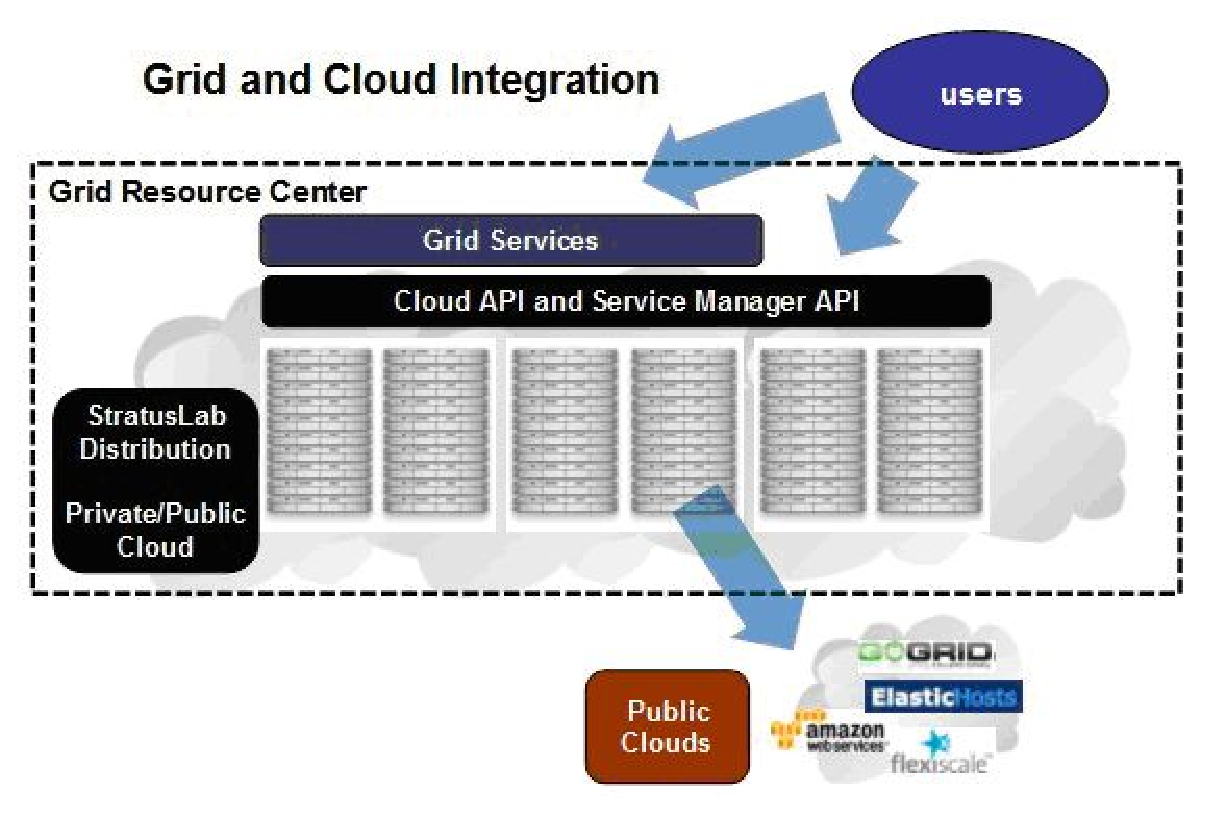
\includegraphics[width=13cm]{fig26.eps} %    ** if .eps don't need extension
\caption{Schema of StratusLab IaaS Cloud interoperability with a
Grid}\label{fig26}
\end{figure}


The basic operations like distributed data management, the high data
throughput and the remote job submission can probably be more
cloud-like. There is a great interest among people to use commercial
Clouds resources, especially when the experiments see their
resources becoming full.

So, can we use Amazon or Google to do processing of data from LHC?
The point is, one cannot be sure what the level of services will be
and what the IN/OUT bandwidth will be. This can in principle be
negotiated with these companies and may bring some level of
agreement. That in principle is doable.


\subsection{Grids and Clouds}

As argued in \cite{Cloud}, "Cloud Computing not only overlaps with Grid
Computing, it is indeed evolved out of Grid Computing and relies on
Grid Computing as its backbone and infrastructure support. The
evolution has been a result of a shift in focus from an
infrastructure that delivers storage and compute resources (in the
case of Grids) to one that is economy based ....". Both the Grids
and the Clouds communities are facing the same problems like the
need to operate large facilities and to develop  methods by which
users/consumers discover, request and use resources provided by the
centralized facilities.

There exist a number of projects looking into and developing Cloud
to Grid interfaces with the idea that Grid and Cloud Computing serve
different use cases and can work together improving Distributed
Computing Infrastructures (see e.g. \cite{Cloud,  Cloud2}). Also CERN is involved
in this activity together with other international laboratories in
Europe.

With the WLCG resources becoming used up to their limits, using
commercial Clouds to process the LHC data is a strategy that should
be assessed. Several of the LHC experiments have done tests whether
they can use commercial Clouds. But today, the cost is rather high.
Also, there are issues like whether academic data can be shipped
through academic networks to a commercial provider or how to make sure
what happens to this data.

Nevertheless the strategy towards deployment over the WLCG resources
Cloud interfaces, managed with high level of virtualization, is
under evaluation. Some level of collaboration with industry would
provide the understanding how to deploy this properly and what would
be the cost. The Cloud and Grid interfaces can be deployed in
parallel or on top of each other. This development might also give a
way to evolve into a more standardized infrastructure and allow to
make a transparent use of commercial Clouds.

A testbed of such an architecture is the CERN LXCloud \cite{LXCLOUD} pilot
cluster. Implementation at CERN allows to present a Cloud interface
or to access other public or commercial Clouds. This is happening
with no change to any of the existing Grid services. Another
interesting example is the development of a comprehensive OpenSource
IaaS (Infrastructure as a Service) Cloud distribution within the
StratusLab project, see Figure 26. Anyone can take the code and
deploy it on his site and have IaaS Cloud running on his site. The
project is focused on deploying Grid services on top of this Cloud,
1) to be a service to existing European Grid infrastructures and to
enable these people to use Cloud-operated resources and 2) because
the developers consider the Grid services very complex and making
sure they run safely on this Cloud should guarantee that also other
applications will run without problems.


\subsection{Physics results achieved by the LHC experiments}

Before we bring the final concluding remarks for our chapter, we
will briefly summarize the Physics results delivered by the LHC
experiments by the time of writing this document.

In addition to many specific new results describing different
Physics phenomena in the energy regime never explored before, there
have been new findings concerning some of the major issues addressed
by the LHC research.

\begin{itemize}
\item ATLAS and CMS experiments have been delivering results concerning
the energy regions excluding the mass of the Higgs boson. The latest
results on the topic of Higgs boson searches exclude a wide region
of Higgs boson masses: ATLAS excludes Higgs boson masses above 145
GeV, and out to 466 GeV (apart from a couple of points in-between,
which are however excluded by CMS studies). For some of the latest
references see \cite{higgs}, \cite{higgs2}, \cite{higgs3}.

\item To contribute new results on the topic of the dominance of matter
over antimatter in the present Universe, the LHCb experiment has
been pursuing studies of phenomena demonstrating the so-called
CP-symmetry violation. Violation of this symmetry plays an
important role in the attempts of Cosmology to explain the dominance
of matter over antimatter in our world. The latest LHCb results
concerning the demonstration of the existence of the CP-violation
can be found e.g. in \cite{cpvio}.

\item The study of properties of the Quark Gluon Plasma (QGP), the phase
of matter which existed in a fraction of a second after the Big
Bang, is the mission of the ALICE experiment. During the lead-lead
collisions at the LHC energies, the individual collisions can be
seen as "little Big Bangs". The matter produced in these collisions
is under extreme conditions: the energy density corresponds to a
situation when 15 protons are squeezed into the volume of one proton
and the temperature reaches more than 200000 times the temperature
in the core of the Sun. ALICE has confirmed the previous findings of
the STAR experiment at the Relativistic Heavy Ion Collider (RHIC) at
Brookhaven that this QGP behaves like an ideal liquid \cite{alice_pbpb} even
at the LHC energies.
\end{itemize}

\subsection{Concluding remarks}

 As we already stressed, the WLCG performance
during the LHC data taking in 2009-2011 was excellent and the basic
mission of the WLCG has been fulfilled: the data taking and
processing is ongoing without major show-stoppers, hundreds of
people are using the Grid to perform their analysis and unique
scientific results are delivered within weeks after the data was
recorded. In addition, the experience gained during this data taking
.stress test. launched new strategies to be followed on the way of
the future WLCG development. There are fundamental issues like the
approaching lack of WLCG resources and the expansion of new
technologies like the Cloud computing. In the time of writing this
paper it looks like we will see in the future some combination of
Grid and Cloud technologies will be adopted to operate the
distributed computing infrastructures used by the HEP experiments.

